\subsectionA{Hej-Kin}
Hej-kin are a race of degenerate humanoids that spend their entire lives underground, dwelling in the Athasian underdark near suitable supplies of water. They are omnivores and subsist largely on a diet of small subterranean creatures and plants.

Hej-kin are malevolent creatures that enjoy inflicting pain and fear on those who trespass on their caverns, blaming them for the damage that has been inflicted on the earth by the defilers.

Hej-kin language is a combination of sign and verbal communication, and their voices are low-pitched, resembling human mumbling. Few surface dwellers are able to learn the language. The color of their skin varies from red to light green, but their skin is always thick and very tough. Hej-kin live on average for 40 or 45 years.

\begin{figure}[t!]
\centering
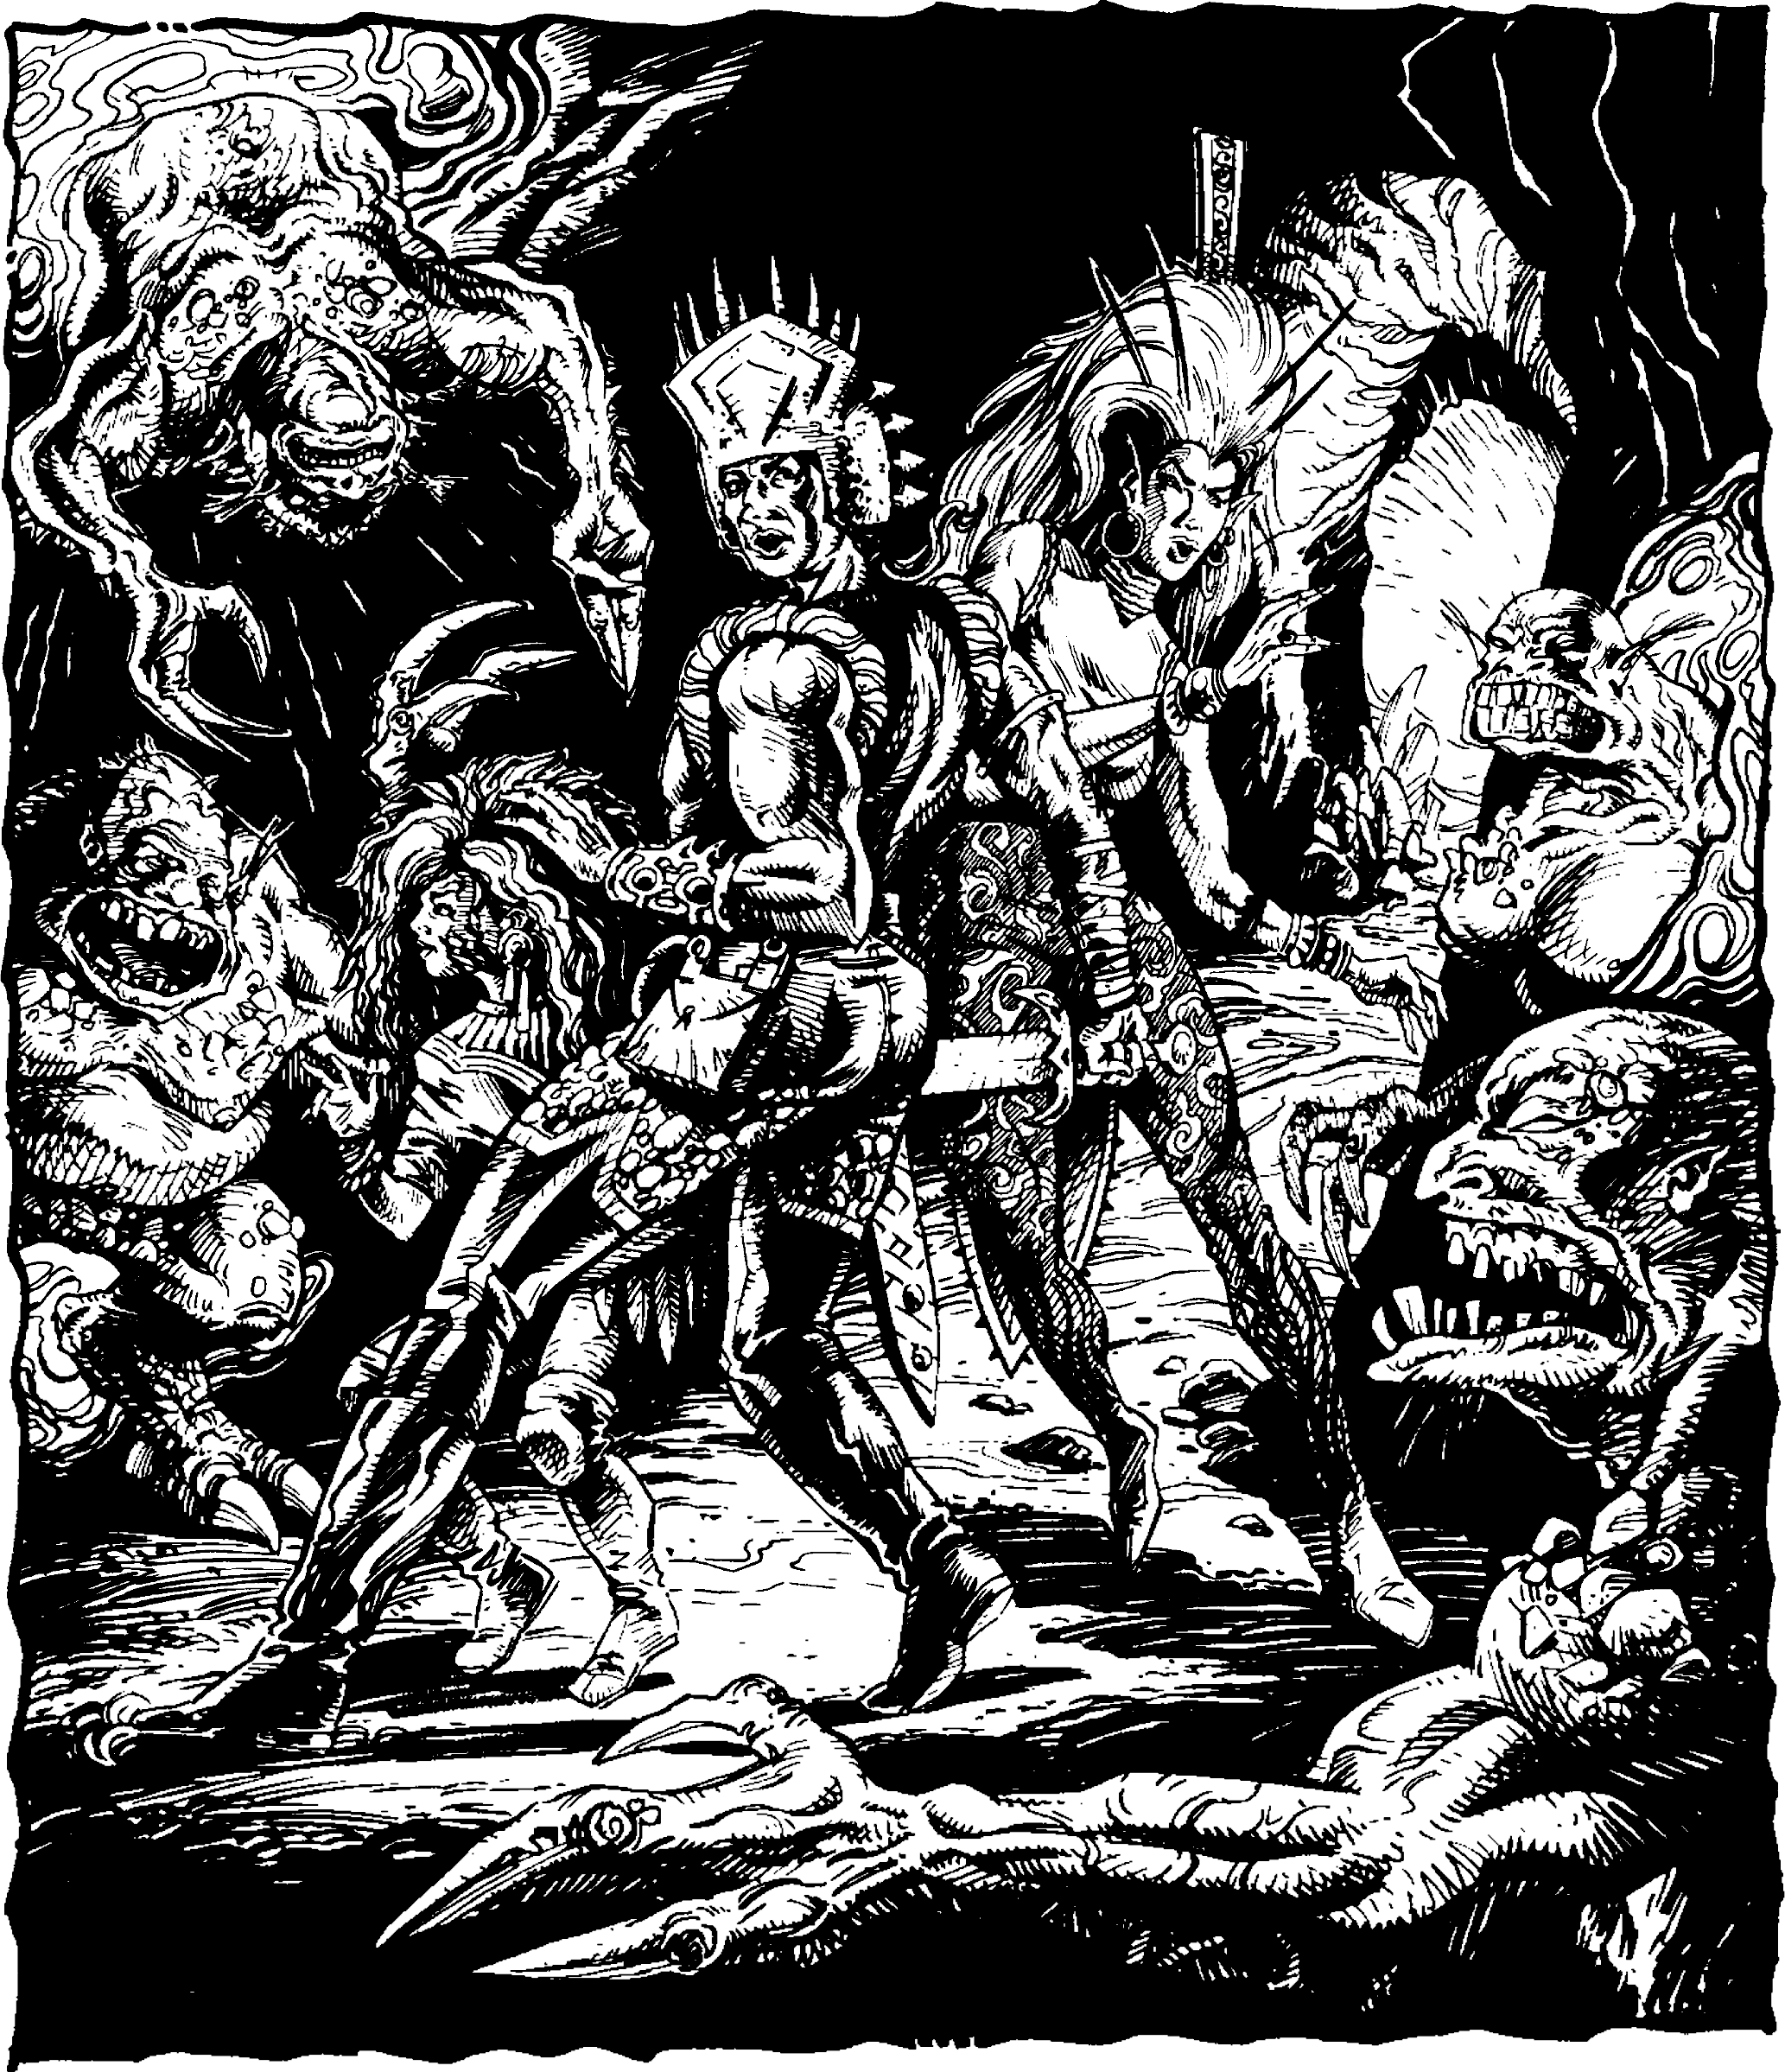
\includegraphics[width=\columnwidth]{images/hej-kin.png}
\WOTC
\end{figure}

\subsubsection{Hej-Kin Society}
Hej-kin do not create artificial tunnels or caves, as they consider the earth to be sacred. They will only occupy naturally-occurring subterranean formations, but they mark these as their property with curious runes on the cave walls.

Hej-kin clans are often led by earth clerics and preservers. Clerics rise highest in hej-kin society and are the only hej-kin who travel to the surface, usually investigating a disturbance that threatens the earth. Hej-kin are never defilers.

Hej-kin are natural enemies to most other surface dwelling and subterranean races, due to the abuse and destruction of the earth perpetrated by these others. Hej-kin clans will migrate to a new area every decade in order to avoid over-using the land on which they dwell.

\subsubsection{Hej-Kin Racial Traits}
\begin{itemize*}
    \item $-4$ Dexterity, +4 Wisdom, $-2$ Charisma: Hej-kin are not agile, and they don't understand the surface dwellers society.
    \item Humanoid (hej-kin): Hej-kin are humanoid creatures with the hej-kin subtype.
    \item Small: Hej-kin gain a +1 size bonus to Armor Class, a +1 size bonus on attack rolls, and a +4 size bonus on \skill{Hide} checks, but they must use smaller weapons than humans use, and their lifting and carrying limits are three-quarters of those of a Medium character.
    \item A hej-kin's base land speed is 6 meters. They may phase through rock and earth at a speed of 3 meters.
    \item Darkvision: Hej-kin can see in the dark up to 18 meters. Darkvision is black and white only, but it is otherwise like normal sight, and hej-kin can function just fine with no light at all.
    \item Racial Hit Dice: A hej-kin begins with 2 levels of humanoid (hej-kin), which provide 2d8 Hit Dice, a base attack bonus of +1, and base saving throw bonuses of Fort +3, Ref +0, and Will +0.
    \item Racial Skills: A hej-kin's humanoid levels give it skill points equal to 5 $\times$ (2 + Int modifier). Its class skills are \skill{Hide}, \skill{Listen}, \skill{Spot} and \skill{Survival}.
    \item A hej-kin's humanoid levels give it one feat.
    \item Weapon Proficiency: A hej-kin is proficient with its natural weapons and all simple weapons.
    \item Natural Armor: +1 natural armor bonus to AC.
    \item Natural Weapons: 2 claws (1d4).
    \item Phase (Ps): Hej-kin may move through earth and rock at a speed of 3 meters. They may stop while inside of walls or floors and remain there indefinitely.
	\item Hej-kin receive a +30 circumstance bonus on \skill{Hide} checks while phased inside solid rock.
	\item Poison (Ex): A hej-kin delivers its poison with a successful claw attack. Fortitude DC 11 + Con modifier. The initial and secondary damage are 1 Con.
	\item Psi-like Abilities: 2/day---\psionic{biofeedback}, \psionic{body equilibrium}, \psionic{claws of the vampire}, \psionic{mindlink}* (three targets), \psionic{thought shield}. Manifester level 3rd. The save DCs are Charisma-based.

	* Includes augmentation for the hej-kin's manifester level.
    \item Automatic Languages: Hej-kin. Bonus Languages: Anakore, Common, Elven, Gith, Tarek.
    \item Favored Class: Rogue.
    \item Level Adjustment: +2.
\end{itemize*}
